\documentclass[12pt]{article}

% Language setting
\usepackage[utf8]{inputenc}
\usepackage[bulgarian]{babel}

% --------------------- Packages  --------------------
% Use biblatex
\usepackage{biblatex}
\addbibresource{bibliography.bib}
% Table thickness
\usepackage{ctable}
% Equations: SI units
\usepackage{siunitx}
% Approximately equal
\usepackage{amssymb}
% degrees symbol
\usepackage{gensymb}
% warning box
\usepackage{pifont,mdframed}
% Multiline math
\usepackage{amsmath}

\newenvironment{warning}
  {\par\begin{mdframed}[linewidth=2pt, linecolor=white]%
    \begin{list}{}{\leftmargin=1cm
                   \labelwidth=\leftmargin}\item[\Large\ding{43}]}
  {\end{list}\end{mdframed}\par}

% --------------------- Title  --------------------
\addbibresource{bibliography.bib}

\begin{document}

% Anfang der Titelseite________________________________________________________________________________
\begin{titlepage}
	\flushleft
	{\scshape\Large Протокол V \hspace{2cm} Молекулна физика\par}
	\vspace{4cm}
	{\huge\bfseries Измерване на относителна плътност на пари по метода на Виктор Майер\par}
	\vspace{1cm}
	{\LARGE\bfseries Лабораторно упражнение №3.5\par}
	\vspace{5cm}
    {\LARGE\bfseries Виолета Кабаджова, \par}
    {\large\bfseries ККТФ, фак. номер: 3PH0600026\par}
	\vspace{1cm}
	
	{\large Физически Факултет, 
	
	Софийски Университет "Св. Климент Охридски"
	
	28 май 2023 г.\par}
	
\end{titlepage}

\section{Теоритична част}\label{sec:theoretical-part}
\underline{Забележка:} \textit{В текущия протокол, макар и нестандартно, ще бележим относителната плътност с $r$} (латинският аналог на гръцкото $\rho$). 

Упражнението цели измерването на относителната плътност на пари хлороформ спрямо плътността на въздух при нормални условия (налягане $p$ = 101 325 Pa и температура $T$ = 273.15 K). Тъй като в повечето случаи абсолютната стойност на газове и пари е много малка, то за удобство плътността се дефинира като относителна плътност между два газа, като най-често използваният еталон е сух въздух при нормални условия. Тази дефиниция се формулира във вида \ref{eq:relative-density-definition}, където $\rho_0$, $V_0$, $M_0$ са съответно плътността, обемът и масата на изследваното вещество, а $\rho_{air}$ - плътността на въздуха.  

\begin{equation}\label{eq:relative-density-definition}
    r = \frac{\rho_0}{\rho_{air}} = \frac{M_0}{V_0} \frac{1}{\rho_{air}}
\end{equation}

\section{Експериментална част}

\subsection{Експериментална установка}
\begin{figure}
    \centering
    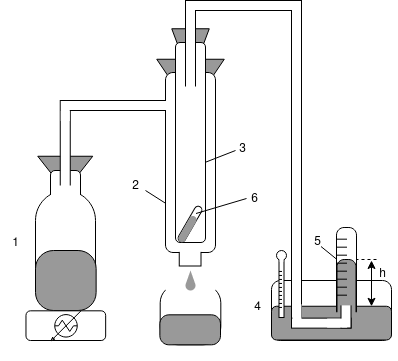
\includegraphics[width=0.5\textwidth]{images/setup-victor-meyer.drawio.png}
    \caption{\label{fig:setup}Схема на опитна постановка; 1 - колба над нагревател, 2 - стъклен кожух, 3 и 4 - стъклени съдове, 5 - измерителна епруветка, 6 - ампула}
    \label{fig:setup}
\end{figure}

Над нагревател се слага стъклена колба пълна с вода, която се загрява и изпарява, като след това поема по тръбичките на системата. Когато парата стигне до стъкления съд 2 на схемата (фиг. \ref{fig:setup}), тя започва да затопля стъкления съд 3, след което да кондензира и да излиза от стъкления кожух 2, падайки в съда отдолу. Когато вътрешния съд 3 се загрява, въздухът в него се разширява и се отвежда до епруветка 5, където избутва част от водата. Следователно в епруветка 5 можем да измерим пряко изместеното количество обем. Отбелязваме, че налягането в епруветката, което съответства на нивото в широкия съд 4, е сума от хидростатичното налягане на стълба вода с височина $h$ над това ниво ($\rho_{H_20}gh$) и налягането на газовата смес в горния край на епруветката, което от своя страна е сума от парциалните налягания $p_1$ на изместения въздух от съда 3 и на наситените пари $e$ ($e$ зависи от температурата на водата в епруветката 5). 

Тъй като съд 4 и епруветка 5 са скачени съдове, и налягането на повърхността на водата в съд 4 е равно на атмосферното налягане $p_{atm}$, то от условието за равновесие на скачени съдове следва ур. \ref{eq:p1}. 

\begin{equation}\label{eq:p1}
    p_{atm} = p_1 + e + \rho_{h_2o}gh,
\end{equation}

\begin{equation}\label{eq:p1}
    p_1 = p_{atm} - e - \rho_{h_2o}gh,
\end{equation}

Работната формула, която ще използваме е формула \ref{eq:work-formula}, където $M_0$, $V_0$, $p_0$, $\rho_0$ са съответно масата, обемът, налягането и плътността на изследваното вещество, $T_{atm}$, $p_{atm}$ - съответните температура и налягане на атмосферата при стандартни условия, $p_1$, $e$ - съответните парциални налягания на изместения въздух от съда 3 (фиг. \ref{fig:setup}) и на наситените водни пари, $\rho_{h_2o}$ - плътността на водата в съд 4 (фиг. \ref{fig:setup}), $h$ - височината на водата в епруветка 5 (фиг. \ref{fig:setup}).

\begin{equation}\label{eq:work-formula}
    r = \frac{\rho_0}{\rho_{air}} = \frac{M_0 T_{air} p_0}{V_0 T_{atm} \rho_{air} p_{1}} = \frac{M_0 T_{air} p_0}{V_0 T_{atm} \rho_{air}} \frac{1}{\left(p_{air} - e - \rho_{h_2o}gh\right)}
\end{equation}

\subsection{Задача: Измерване коефициента на вътрешно триене и дължината на свободния пробег на молекулите на въздуха}
Правим експеримента веднъж и записваме измерванията в таблица \ref{tbl:results}. За да намерим масата на изследваното вещество, използваме формула \ref{eq:mass-ch}, където $V_{ch}$ е първоначално налятото количество хлороформ в ампула 6 на фиг. \ref{fig:setup}. Използваните стандартни константи записваме в таблица \ref{tbl:constants}, като тяхната грешка е половината от най-малкото записано деление.

\begin{equation}\label{eq:mass-ch}
    M = V_{ch}\qho_0 = 1489 \cdot 4 \cdot 10^{-9} = (60 \pm 7) \cdot 10^{-6} kg    
\end{equation}

\begin{table}[h]
\begin{center}
\begin{tabular}{|l|l|l|l|l|} \hline
    Величина & Стойност и грешка & Мерна единица \\ \hline
    Плътност на въздуха $p_{air}$ & 95 389 \pm 10 & Pa \\ \hline
    Температура на въздуха $T_{air}$ & 292 \pm 0.5 & K \\ \hline
    Плътност на хлороформ $\rho_0$ & 1489 \pm 0.5 & kg/m^3 \\ \hline
    Налято количество && \\
    хлороформ в ампула $V_{ch}$ & (40 \pm 5) \cdot 10^{-6} & m^3 \\ \hline
    Обем газ в епруветка $V_0$ & (7.5 \pm 0.05) \cdot 10^{-6} & m^3 \\ \hline
    Височина на воден стълб && \\
    в епруветка $h$ & (9 \pm 0.5) \cdot 10^{-2} & m \\ \hline
    Налягане на наситени & & \\
    водни пари при 19 \deg C $e$ & 2199.45 \pm 24 & Pa \\ \hline
\end{tabular}
\caption{\label{tbl:results}Измервания и резултати}
\end{center}

\end{table}
\begin{table}[h]
\begin{center}
\begin{tabular}{|l|l|l|} \hline
    Величина & Стойност & Мерна единца \\ \hline
    Атмосферно налягане && \\
    при нормални условия $p_{atm}$ & 101 325 & Pa \\ \hline
    Температура при && \\
    нормални условия $T_{atm}$ & 273.15 & K \\ \hline
    Плътност на въздуха $\rho_{air}$ & 1.293 & kg/m^3 \\ \hline
    Земно ускорение $g$ & 9.81 & m/s^2 \\ \hline
    Плътност на водата $\rho_{h_2o}$ & 997 & kg/m^3 \\ \hline
\end{tabular}
\caption{\label{tbl:constants}Използвани стандартни константи}
\end{center}
\end{table}


 Използвайки ур. \ref{eq:work-formula}, получаваме $r$ = 7.2 $\pm$ 1.4. Тъй като относителната плътност $r$ е съотношение между две други плътности, то тази величина е безразмерен коефициент. 

\end{document}
